\documentclass[11pt, oneside]{article}   	% use "amsart" instead of "article" for AMSLaTeX format
\usepackage{geometry}                		% See geometry.pdf to learn the layout options. There are lots.
\geometry{letterpaper}           
\usepackage[parfill]{parskip} 
\usepackage{graphicx}	
\usepackage{amssymb}
\usepackage{amsfonts}
\usepackage{amsmath}
\usepackage[latin1]{inputenc}
\usepackage{float}
\renewcommand{\abstractname}{}

%\newcommand*{\R}{\mathbb{R}}
%\newcommand*{\abs}[1]{{\lvert#1\rvert}}
%\newcommand*{\Abs}[1]{{\Big\lvert#1\Big\rvert}}
%\newcommand*{\ABS}[1]{{\left\lvert#1\right\rvert}}
%\newcommand*{\set}[2]{{\{#1 \mid #2\}}}
\def\i{\hat{\imath}}
\def\dt{\Delta t}
\def\dtm{\Delta t_{\mathrm{max}}}

\title{Gravitational $N$-Body Simulations}
\author{Gudbrand Tandberg}
\date{\today}							% Activate to display a given date or no date

\begin{document}
%====================MAIN PAPER==============================
\maketitle
\thispagestyle{empty}
%\newpage

%====================Section 1==============================
\begin{abstract}
In this article we will study the numerical modelling of gravitationally interacting $N$-body systems. The first part of the article focuses on introducing the subject matter and presenting some of the results of the simulations. The numerical methods are first explained and then tested on the simple model consisting of the inner solar system. We then proceed to present a upgraded version of the solver featuring adaptive timesteps and parallellization. The simulations of the inner solar system are re-run and compared with the ones previously obtained. In the second part of the article we turn our attention to increasing $N$. We use as our physical system that of a uniform spherical distribution of point-masses at rest. This system could for example model a small cluster of stars. We study some pf the physics of such a system and also consider some numerical aspects of increasing $N$.

All the programs, animations and articles refered to in the paper can be found at http://github.com/gudbtandberg/N-Body.
\end{abstract}

\section*{Foreword}



\section{Introduction to the $N$-body problem}

We start off by giving the basic definition of the problem to be solved. The system consists of $N$ point-masses moving in space under the influence of mutual gravitational forces. Denote the mass, position and velocity of body $i$ as $m_i, r_i$ and $v_i$ respectively (the latter two being three dimensional vectors). According to Newton, the gravitational acceleration on body $i$ is given by

\begin{equation}
a_i = \sum_{j\neq i}\frac{Gm_j}{r_{ij}^2}\i_{ij},
\label{gravity}
\end{equation}

where $r_{ij}$ is the distance between body $i$ and $j$, $G$ is the gravitational constant and $\i_{ij}$ is the unit vector pointing from body $i$ towards body $j$. This can be used to determine the differential equations of motion for all the particles, by decoupling Newton's second law as a system of ordinary first order differential equations.

\begin{equation}
\begin{bmatrix}
r_i \\
v_i \\
\end{bmatrix}'
= 
\begin{bmatrix}
v_i�\\
a_i \\
\end{bmatrix}.
\label{diffeq}
\end{equation}

From now on we refer to the couple $(r, v)$ as the \emph{state} of a body. All in all this gives us one 6-dimensional coupled ordinary differential equation for each body, or $6N$ ordinary differential equations. All that is needed to simulate such a system for any descretized period of time $T$ is the initial positions and velocities of all of the bodies along with a rule for how to move the system from one time to the next. Such rules will be dicussed further in the next section.

\subsection{Scaling the equations}

In the problem set forth in the previous section we saw that there were 3 different units of measurement; length, time and mass. To simplify the numbers involved in a simulation, the equations should be scaled appropriately. In the case of the solar system, the natural unit of length is the astronomical unit, defined to be the mean distance between the Sun and the Earth; approximately $1.49\cdot 10^{11}$ m. We arbitrarily choose one week as our unit of time, or $60\cdot60\cdot24\cdot7$ s. We could fix the unit of mass to be the mass of the Earth or Sun, but instead choose the mass scale so as to fix $G = 1$. This is equivalent to fixing the unit of mass. In scaling the equations, what we are really doing is performing the change of variables

\begin{eqnarray}
r \to \frac{r}{r^*} \\
t \to \frac{t}{t^*} \\
m \to \frac{m}{m^*} \\
\end{eqnarray}

where $r^*, t^*$ and $m^*$ are the characteristic lengths of the units involved. To find out what our characteristic mass will be, we first note that the unscaled value of $G$ in SI-units is $G = 6.67\cdot10^{-11} \mathrm{m}^3/\mathrm{kg}\cdot\mathrm{s}^2$. Denoting the scaled value of $G$ by $G^*$, we get that

\[
G^* = \frac{6.67\cdot10^{-11} \mathrm{m}^3/\mathrm{kg}\cdot\mathrm{s}^2\cdot m^*\cdot{t^*}^2}{{r^*}^3}
\]

Setting this equal to one and solving for $m^*$ yields

\[
m^* = \frac{{r^*}^3}{6.67\cdot10^{-11}\mathrm{m}^3/\mathrm{kg}\cdot\mathrm{s}^2 {t^*}^2}
\]

In our case

\[
m^* = \frac{\mathrm{AU}^3}{6.67\cdot10^{-11}\mathrm{m}^3/\mathrm{kg}\cdot\mathrm{s}^2\cdot\mathrm{week}^2} = x \mathrm{kg}
\]

The only point in the program where the units come into the picture are in the setting up of the initial conditions. All values in the input files for the inner solar system are in these units. 

\subsection{A brief history the N-Body problem}

For the simple case of $N=2$, closed form analytical solutions to the problem defined by \eqref{gravity} and \eqref{diffeq} exist. In fact, these solutions were first discovered by Newton himself. The idea in his solution consists of a series of simplifications; first eliminating some unknowns by changing coordinates to the centre of mass coordinates, then using conservation of angular momentum to assert that all the motion will be in a plane to eliminate 4 more unknowns. Finally, the trajectories of the bodies can be shown to follow conic sections. This result is consistent with Kepler's earlier discovery that bound planets move in ellipses, and unboud bodies move in hyberbolic or parabolic trajectories. This must have motivated Newton to take on the three-body system, which he did in his lunar investigations in Principia. But no general solutions were found. 

Finding analytical solutions of the three-body problem stood unsolved for over two centuries untill Poincar� showed that there is no general closed form solution to the three-body problem. Furthermore it was shown by him that the trajectories are generally non-repeating, or chaotic in modern terms. This must have shocked the scientific community, shattering (not for the last time) any idea of a 'clockwork universe'. 

Poincar�'s discovery did not however halt further research into the three-body problem. Further contributions to the problem were put forward by Lagrange, Liouville, Laplace, Jacobi, Darboux and Hamilton amongst others. It was discovered that in many special cases closed form solutions do exist. At the time of writing 16 families of solutions to the three-body problem are known. 13 of these were discovered in 2013.

With the advent of computers in the middle of the 20'th century, the $N$-body problem could finally be studied in further detail for $N > 3$. As computing power increased exponentially, larger and larger systems could be studied. Today, large $N$ simulations are used as tools in astrophysics and cosmology to study concepts such as the evolution of star clusters, or even the evolution of the large scale structure of the universe. A modern example of such a simulation is the so-called Millenium Run, where the trajectories of $2160^3$ (just over 10 billion) bodies were computed. The computation lasted over a month on a super computer in Switzerland. 

\section{The numerical methods}

In this section we present the two different methods used to move the bodies forward in time, so-called integration schemes. The two methods we will use are the Velocity Verlet method and the fourth order Runge Kutta method. We assume we are at a time $t$, where the quantities $r(t)$ and $v(t)$ are known, and we wish to determine $r(t+\dt)$ and $v(t+\dt)$. In the following derivations we only consider the state of one body and adopt the notation $r_i = r_i(i\dt), v_i = v(i\dt)$, where $i = 1, \cdots, n, $and $\dt$ is the time step. 

\subsection{The Velocity Verlet method}

The first integration method we utilize in our simulations is the \emph{Velocity Verlet} method. It is characterized by the equations

\begin{eqnarray}
v_{i+1/2} = v_i + a_i\dt /2\\
r_{i+1} = r_i + \dt v_{i+1/2}\\
v_{i+1} = v_i + \dt\frac{a_i + a_{i+1}}{2}
\end{eqnarray}

First we compute a better approximation to the velocity at time $i$ by using the computed value $v_{i+1/2}$. This will be recognized as the Taylor expansion of the velocity at time $i$ truncated to second order. This value is then used to compute the position at time $i+1$. To compute the value of the velocity at time $i+1$ the acceleration at time $i+1$ is first computed using the newly found positions at time $i+1$. The velocity is then set to the current velocity plus the time step times the average acceleration between time $i$ and time $i+1$. We note that only one force evaluation is necessary at each step, since the acceleration $a_{i+1}$ found at any time can be stored and used as $a_i$ in the next step. We do not derive the order of the error terms, but simply state the fact that the local error (the error that occours when stepping from one timestep to the next) is of order $O(\dt^4)$ in position, but only of order $O(\dt^2)$ in velocity. The global error (the accumulated error after many timesteps is of order $O(\dt^3)$. It shall be interesting to observe these facts in the simulations presented later on. 

As an aside we can mention that the Verlet integration scheme has the nice properties of being a sympleptic and time-reversible scheme, meaning that it conserves the energy of the system well, and it can be run backward and return exactly to a earlier initial condition. These are for obvios reasons desirable properties when solving the $N$-body problem.

\subsection{Runge Kutta 4}

\section{The first NBodySolver class}

In this section we describe the basic behaviour of the first $N$-body solver used in the simulations. The program can be found in \verb+source/NBodySolver.cpp+ in the main project page. The program uses a object-oriented structure, the main objects being \verb+NBodySolver+, and \verb+Body+. The former acts as the controller object. It is initialized as \verb+NBodySolver(N, T, dt, method)+. Methods for initializing, solving and finally writing the results to files are all called from a main program, in our case \verb+main.cpp+. 

The most important attribute of the NBodySolver class is the list of bodies; \verb+bodies+. Each body has attributes \verb+r+ and \verb+v+ corresponding to the position and velocity at the present time. In addition, each body keeps track of the positions and velocities at all previous times in the matrix \verb+state_history+. This matrix is incrementally updated at each pass of the main integration loop.

The integration loop, implemented in the \verb+solve()+-method is the most central part of the program. In pseudocode, the algorithm is as follows

\begin{verbatim}
while global time < T
    extract the states of all the bodies
    step all planets using either Verlet of Runge Kutta
    update positions and velocities of bodies
    global time++
\end{verbatim}

There are of course some technicalities regarding the specific implementations of the different integration methods, but the explanation of these are left to the comments.

After the integration loop is finished, the main program calls the \verb+writeTrajectories()+ and \verb+writeEnergy()+ methods of the solver. As this project features a lot of output a necessarilly cumbersome naming convention was adopted for filewriting: 

\begin{verbatim}
N_body_type_T_dt_adaptive_method_cpus_eps.dat,
\end{verbatim}

where \verb+type+ is either energy or trajectories, \verb+N, T+ and \verb+dt+ are obvious, \verb+adaptive+ is either 0 or 1, \verb+method+ is either 0 (Verlet) or 1 (RK4), and \verb+cpus+ and \verb+eps+ are the number of cpus to be used and the smoothing factor respectively, to be explained in a later section. 

\section{Results for the solar system}

\begin{figure}[H]
\begin{center}
\caption{Solar system trajectories integrated with the Velocity Verlet method over one Giovian year using three different timesteps}
\label{}
\end{center}
\end{figure}


\begin{figure}[H]
\begin{center}
\caption{Solar system trajectories integrated with the fourth order Runge-Kutta method over one Giovian year using three different timesteps}
\label{}
\end{center}
\end{figure}

\begin{figure}[H]
\begin{center}
\caption{Evolution of the total mechanical energy of the inner solar system using the Verlet method}
\label{}
\end{center}
\end{figure}

\begin{figure}[H]
\begin{center}
\caption{Evolution of the total mechanical energy of the inner solar system using the fourth order Runge Kutta method}
\label{}
\end{center}
\end{figure}

\begin{table}[H]
\begin{center}
\begin{tabular}{c|c|c}
$\dt$ & Velocity Verlet & RK4 \\
\hline
2.0 & 15995 & 33335 \\
1.0 & 41919 & 81971 \\
0.1 & 2223195 & 2596803 \\
\end{tabular}
\end{center}
\label{}
\caption{Time taken to integrate the inner solar system (6 bodies) using the different integration methods}
\end{table}


\section{Extending the NBodySolver}

In this section we describe how we can change the solution algorithm and implementation to allow for adaptive timesteps and parallellization using OpenMP. 

A slight drawback when it comes to allowing these changes is that some major ideas in the implementation of the last NBodySolver have to be altered. This makes the comparison of the two different approaches slightly more nuanced, but for the most part we ignore these difficulities when they arise. 

The new solver, found in \verb+APNBodySolver.cpp+, is nonetheless quite similar to the normal \verb+NbodySolver+ object. The solver is initialized as \verb+APNBodySolver(N, T, dtmax, epsilon, cpus)+. As before, there are methods for reading input files and initializing, solving and writing the results to files. We first discuss the adaptive solution algorithm. 

\subsection{Adatpive step sizes}

The evolution of an arbitrary $N$-body system is in most cases characterized by several different timescales. For instance, in the inner solar system change happens much more rapidly for Mercury than for Jupiter, and even more so for Mars' moon Phobos, which orbits Mars in just over 7 hours. Even in a cluster of stars, for any given star, there will be time periods in which the motion is smooth and slow, and there will be periods where the state of the star changes very rapidly, for example during a close encounter with another star, or during the formation of a binary system. For this reason it is desirable to allow each body to use a different time step than the other bodies, and also to be able to change its time step along the path of integration.

The most general approach of allowing each body to move forward with its own unique timestep all the time would be very difficult to implement, and perhaps also quite costly computation-wise. A simpler and much more widely used technique is quantizing the allowed timesteps. Using this method, we take as input the maximum allowed timestep $\dtm$, and the number of timesteps $n$. We then define the allowed timesteps to be

\begin{equation}
\dtm, \frac{\dtm}{2}, \dots, \frac{\dtm}{2^{n-1}}.
\end{equation}

To simplify implementation, we choose $n = 3$. This is arguably too few time steps for a significant speedup, but we accept that fact in order to keep the implementation simple. Thus we have three time scales $\dtm, \dtm/2$ and $\dtm/4$. Another constraint we enforce upon the time steps is that a body may only change its time step at times corresponding to integer multiples of $\dtm$. This also in order to simplify implementation. One could ask if this is a reasonable constraint, to which the answer must be that this depends greatly upon the value of $\dtm$. If $\dtm$ is kept small enough, dramatic change within each main time step will be kept to a minimum. [CHANGE VALE OF $\dtm$?]. A final simplification is that we only use the Velocity Verlet method of integration. As we saw in the previous section, this method is good enough for our needs, and is much easier to implement. Unfortunately, the Verlet method loses its property of time reversibility when adaptive time steps are allowed. For a interresting solution to this problem, see \cite{adaptive}. 

The solution algorithm of the \verb+APNBodySolver+ can be described in pseudocode as

\begin{verbatim}
determine the initial timestep of each of the bodies
while global time < T
    twice do
        twice do
            update states of bodies using timestep dtmin
            global time++
        update states of bodies using timestep dtmed
    update states of bodies using timestep dtmax
    compute new timesteps for all the bodies

\end{verbatim}

The order of updating the states of the bodies can be depicted pictorially as in figure \ref{steps}.

\begin{figure}[htbp]
\begin{center}
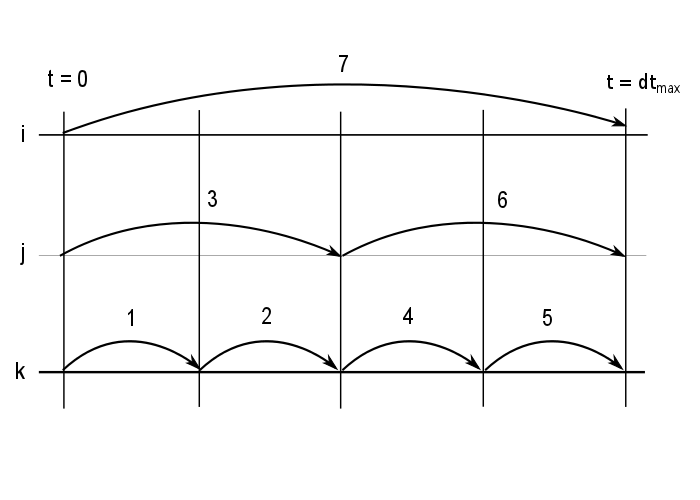
\includegraphics[width=12cm]{./figures/steps.png}
\caption{The order of updating the bodies using the time steps $\dtm$, $\dtm/2$ and $\dtm/4$. The numbers above each arrow tells the order of computations.}
\label{steps}
\end{center}
\end{figure}

A very important implementation detail when using this scheme is hidden away in the pseudocode statement \verb+update states of bodies using timestep dt*+. We noe explain how this step is taken. First, when updating the states of the bodies using the smallest timestep we need to know the value of $a_{i+1}$ for these bodies. This in turn depends upon the positions of \emph{all} the bodies at this timestep. We find these by extrapolating the positions of all the other planets to time $t + \dt_{\mathrm{min}}$. The bodies with larger timesteps are simply moved the correct amount along their current \verb+v_half+ vector. These extrapolated positions are not added to the \verb+state_history+ of the bodies. When going on to compute new states for the bodies using time step $\dt_{\mathrm{med}}$, we can use the current (newly updated) positions of the planets using the smallest time step. The bodies using the largest time step still need to be extrapolated. This is done in the same manner, this time moving $\dt_{\mathrm{med}}$ steps along their \verb+v_half+. Now new states are added twice for the bodies using the medium time step, in order to stay synchronized in time with the other bodies. Finally when computing new states for the bodies using the largest timestep we may use the current positions of all the other bodies along with extrapolated positions of the bodies themselves. New states are added four times for these bodies in order to stay synchronized in time. Although $a_{i+1}$ will always depend upon the positions of \emph{all} the planets at any given time, the function \verb+gravity(states)+ is written in such a way as only to return the gravitational acceleration on the bodies using the time step corresponding to the value of \verb+current_dt+.   

The implementation found in \verb+APNBodySolver+ has several weaknesses. A lot could be done to improve the speed of the integration loop as a lot of time is spent simply moving data around, and also several values are computed many times. In return the implementation is easy to understand and the basic idea of using adaptive time steps gets across. If I were to start over I would definitely omit object orientation of the bodies. This seems to me unnecessary encapsulation of data, and going over to a more purely matrix based implementation would have many benefits. Also allowing more time steps would definitely be worth spending some time on. This could be achieved by altering the algorithm presented above with more clever loops and use of modular arithmetic to synchronize and extrapolate nicely.

\section{Refined results for the solar system}
 
Same simulations as above. Also a discussion of parallellization. 

\subsection{OpenGL animation}

As a fun application of the trajectories generated, a 3D animation of the inner solar system was implemented using the OpenGL library. The planets are modelled as textured spheres revolving around the sun. The relative sizes and rotation periods are not to scale, but the trajectories are accurate. The program can be found in \verb+source/OpenGL_solarsystem.cpp+ of the main project page. A executable compiled on a Macbook Pro running OSX 10.9.5 can also be found there. On other architectures the executable should be compileable by running \verb+make solar_animation+ in a terminal. We do not go into implementation details as the code should speak for itself. 

\begin{figure}[H]
\begin{center}
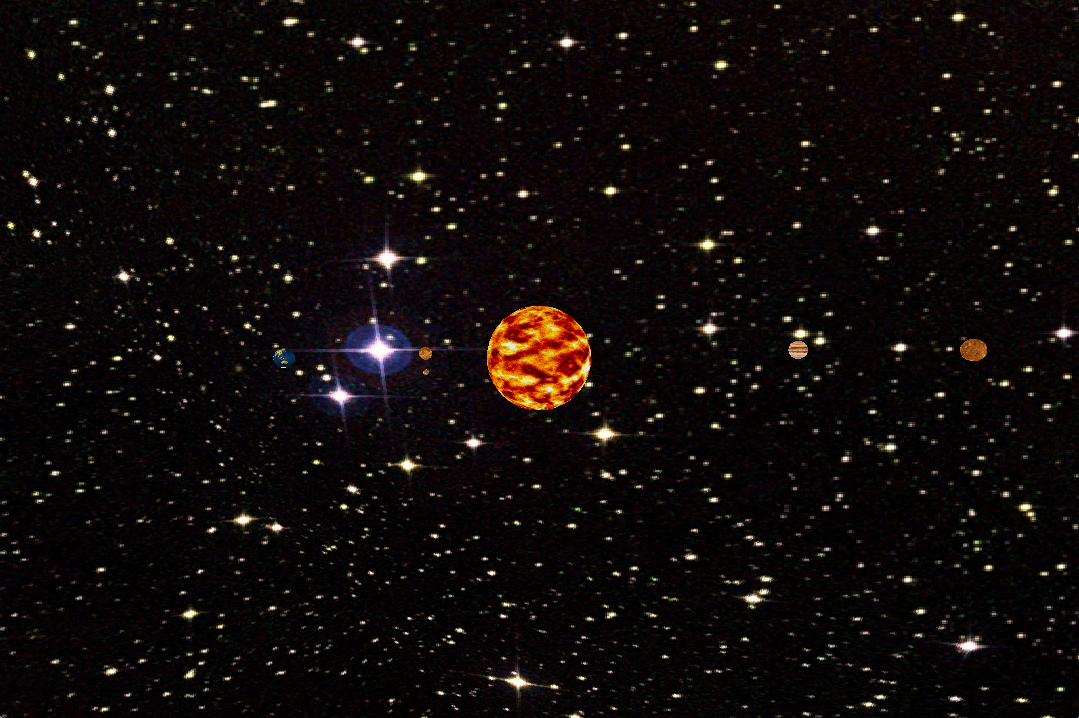
\includegraphics[width=12cm]{./figures/ISS_screenshot.png}
\caption{Screenshot of a run of solar\_animation. From left to right we see Earth, Venus, Mercury, Sun, Jupiter and Mars.}
\label{default}
\end{center}
\end{figure}


\section{Further development of the algorithm}

As wee have seen, the final \verb+APNBodySolver+ is quite an advanced and capable solver. Before moving on to our final application of the solver we take a moment to consider what more could be done to beef up the solver. 

\subsection{Faster gravity evaluations}

The brute-force method of computing the mutual gravitational attraction between $N$ bodies is a $\mathcal{O}(N^2)$ computation. However there are different ways around this costly computation. One of the more popular is the so-called Barnes-Hut tree-method. This way of computing gravitational attraction is of order $\mathcal{O}(N\log N)$. The method is very neat, and we give a summary of it here. At each gravity evaluation, the volume of integration is first subdivided into eight equal subcells. These subcells are then recursively subdivided until only one body is present in each cell. This gives rise to a oct-tree of subcells; starting at the root node consisting of the entire intagration volume, each descendent will either be a cell containing many bodies and eight descendents of its own, or it will be a cell containing only one body. This tree has to be generated at each gravity evaluation. To compute the gravitational attraction on a body, the tree is traversed from the root node, and if the centre of mass of any other cell is far enough away from the body in question, all the bodies in this cell are considered as one particle located at the centre of mass of this cell. By changing what is meant by 'far enough', the accuracy of the computation varies. If 'far enough' is set to infinity, the algorithm collapses into the brute force evaluation. For more on the Barnes-Hut tree code, see \cite{barneshut} 

\subsection{Smoothing factor}

When simulating large $N$ systems, it often occurs that two or more bodies move arbitrarily close to each other. Thus we often experience the singularity at $r_{ij} = 0$ in \eqref{gravity}. This is both physically and numerically a undesirable effect, that can easily be cured. Physically, because in most cases we are not interrested in point-masses, but rather distributions of mass in space. In fact a 'body' in a simulation could be understood to represent several stars and interstellar dust in some cases. So there are several physical reasons to remove the singularity. Numerically it is undesirable because the effect often is that bodies are 'flung' out of the integration domain and really do the simulation no good after this point. There are several ways of removing the singularity, one particularily simple method is perturbing Newtons' equation slightly to read

\begin{equation}
a_i = \sum_{j\neq i}\frac{G m_j}{r_{ij}^2 + \epsilon^2}\i_{ij}
\end{equation}

This modification is actually implemented in \verb+APNBodySolver+, and the value of $\epsilon$ can be given as input to the solver (typically a small number). We study the effect of varying $\epsilon$ in the final section. 

\section{Application: cold cluster collapse}
\subsection{Introduction}
\subsection{Results}
OpenGL animation, discussion on $t_{\mathrm{crunch}}$, virial energy computation, different smoothing \&c. 

\section{Afterword}

%====================BIBLIOGRAPHY===========================
\begin{thebibliography}{9}

\bibitem{github}
	http://github.com/gudbrandtandberg/N-Body

\bibitem{adaptive}
	'A Time-Symmetric Block Time-Step Algorithm for N-Body Simulations'\\
	Junichrio Makino, Piet Hut, Murat Kaplan, Hasan Saygin\\
	\emph{New Astron.} 12 (2006) 124-133

\bibitem{barneshut}
	'A hierarchical O(N logN) force-calculation algorithm'\\
	Josh Barnes \& Piet Hut\\
	\emph{Nature} vol. 324 

\end{thebibliography}


\newpage
\section{Lenker}
http://en.wikipedia.org/wiki/Barnes\%E2\%80\%93Hut\_simulation\\
http://en.wikipedia.org/wiki/N-body\_simulation\\
http://trekto.info/n-body-simulation\\
http://en.wikipedia.org/wiki/Plummer\_model\\
http://burtleburtle.net/bob/math/multistep.html\\
http://www.artcompsci.org/
http://www.ifa.hawaii.edu/faculty/barnes/treecode/treeguide.html\\
https://www.ids.ias.edu/~piet/act/comp/algorithms/starter/

\end{document}  